\documentclass[4pt]{standalone}

\usepackage{tikz}
\usetikzlibrary{calc}

\begin{document}
	
	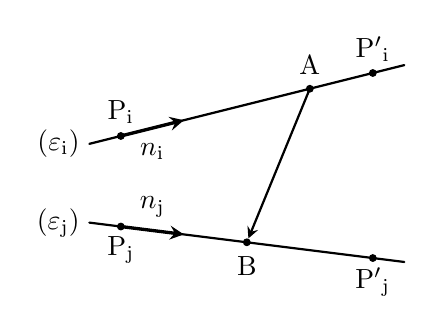
\begin{tikzpicture}[line cap=round]
%		% Grid
%		\draw (0,0) grid (5,5);
%		\foreach \i in {0,1,...,5}
%		{
%			\node at (-1ex, \i) {\i};
%			\node at (\i, -1ex) {\i};
%		}
		
		% Coordinates
		\coordinate (A) at (0,2);
		\coordinate (A') at (4,3);
		\coordinate (AA) at ($(A)!0.7!(A')$);
		\coordinate (a) at ($(A)!0.1!(A')$);
		\coordinate (a') at ($(A)!0.9!(A')$);
		\coordinate (aa) at ($(A)!0.3!(A')$);
		\coordinate (B) at (0,1);
		\coordinate (B') at (4,0.5);
		\node[inner sep=1.2] (BB) at ($(B)!0.5!(B')$) {};
		\coordinate (b) at ($(B)!0.1!(B')$);
		\coordinate (b') at ($(B)!0.9!(B')$);
		\coordinate (bb) at ($(B)!0.3!(B')$);
		
		% Lines
		\draw[thick] (A) -- (A');
		\draw[thick] (B) -- (B');
		
		% Arrows
		\draw[very thick, -stealth] (a) -- (aa);
		\draw[very thick, -stealth] (b) -- (bb);
		\draw[thick, -stealth] (AA) -- (BB);
		
		% Points
		\draw[fill=black, draw=black] (a) circle (1.2pt);
		\draw[fill=black, draw=black] (a') circle (1.2pt);
		\draw[fill=black, draw=black] (b) circle (1.2pt);
		\draw[fill=black, draw=black] (b') circle (1.2pt);
		%
		\draw[fill=black, draw=black] (AA) circle (1.2pt);
		\draw[fill=black, draw=black] (BB) circle (1.2pt);
		
		% Nodes
		\node[left] at (A) {($\varepsilon_\mathrm{i}$)};
		\node[left] at (B) {($\varepsilon_\mathrm{j}$)};
		%
		\node[shift={(0,0.3)}] at (a) {$\mathrm{P}_\mathrm{i}$};
		\node[shift={(0,0.3)}] at (a') {$\mathrm{P'}_\mathrm{i}$};
		\node[shift={(0,-0.3)}] at (b) {$\mathrm{P}_\mathrm{j}$};
		\node[shift={(0,-0.3)}] at (b') {$\mathrm{P'}_\mathrm{j}$};
		%
		\node[shift={(0,-0.3)}] at ($(a)!0.5!(aa)$) {$n_\mathrm{i}$};
		\node[shift={(0,0.3)}] at ($(b)!0.5!(bb)$) {$n_\mathrm{j}$};
		%
		\node[shift={(0,0.3)}] at (AA) {$\mathrm{A}$};
		\node[shift={(0,-0.3)}] at (BB) {$\mathrm{B}$};
	\end{tikzpicture}
	
\end{document}
